\chapter{Der QHScompiler} \label{cha:4-QHS_Compiler}
Die QHS Programmiersprache besteht aus Wörtern. Im Kontext von QHS werden diese Wörter \textit{Orders} genannt. Diese Orders weisen drei verschiedenen Typen auf. \textit{Identifiers}, \textit{Instructions} und \textit{LiteralCode}.
Bei Identifiers handelt es sich um die in Abschnitt \ref{cha:3-Meine_Idee} CHANGE THIS bereits erwähnten Macros. Instructions sind einfache vorprogrammierte Anweisungen an den QHScompiler und LiteralCode ist Text, der unverändert
in die Outputdatei geschrieben wird. Wie diese drei Order Typen genau funktionieren wird in Abschnitt \ref{sec:qhs-execute} ausführlicher erklärt.

Dem QHScompiler steht für die Kompilierung ein einfacher Zyklus zugrunde, dessen Vorbild der Von-Neumann Zyklus ist.

\begin{figure}[h!]
    \centering
    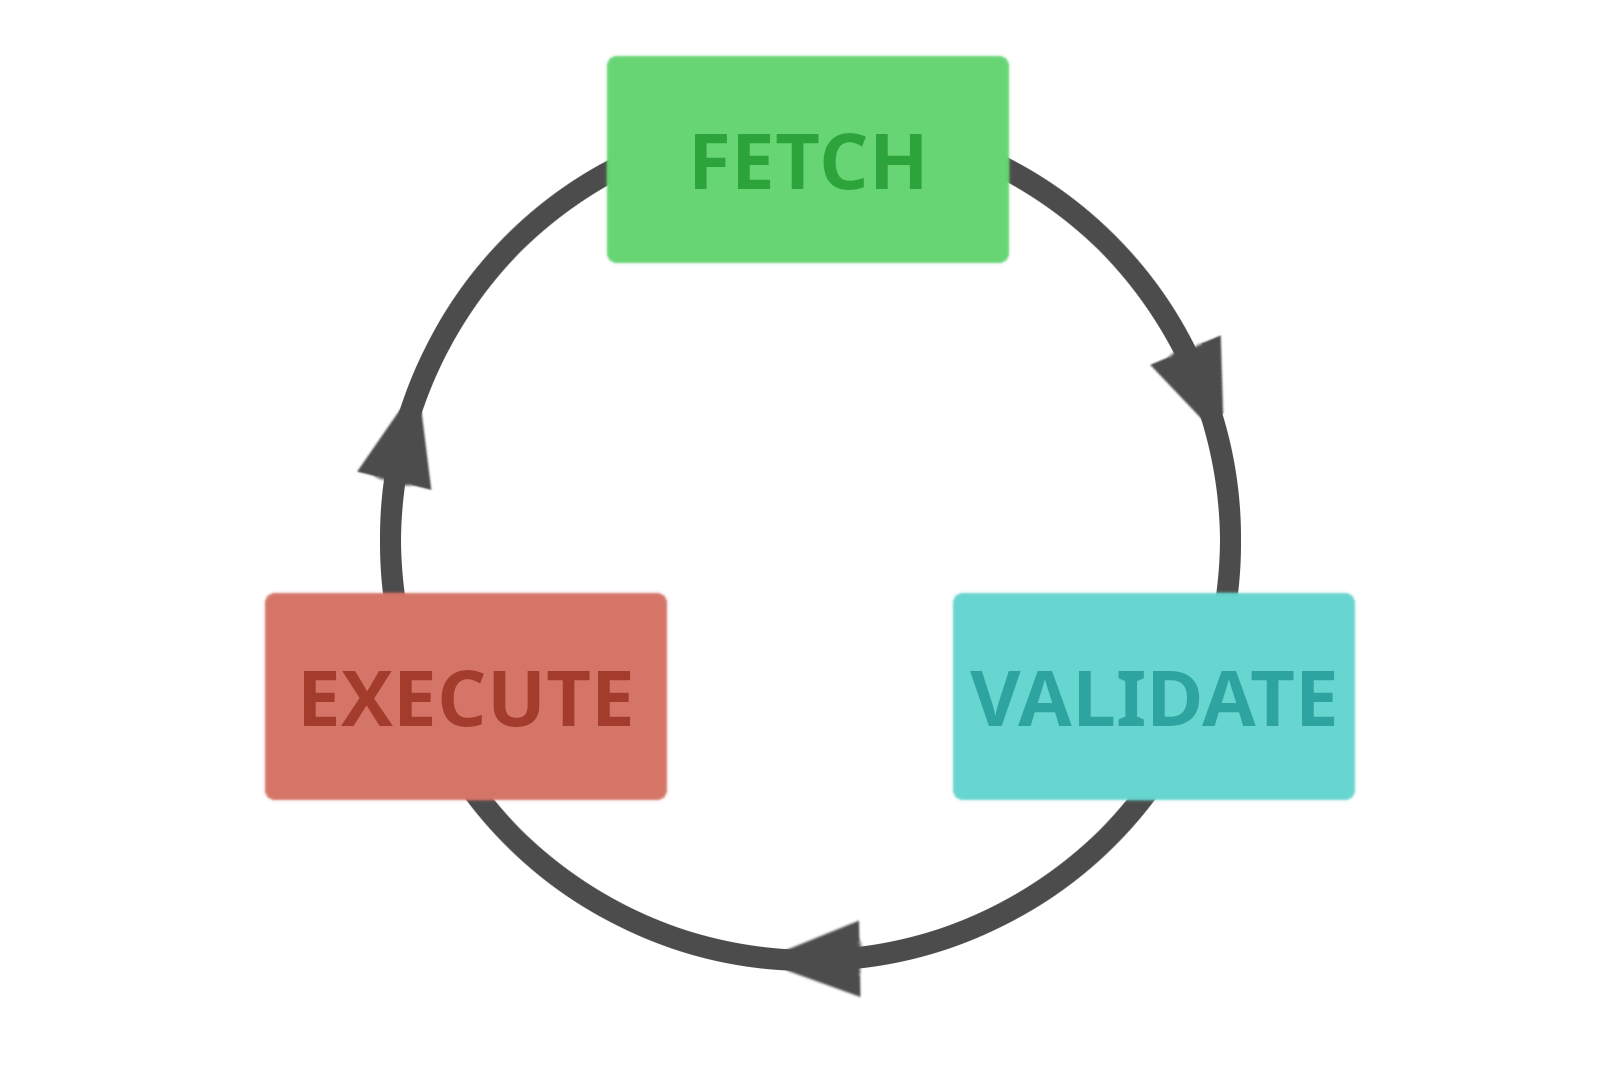
\includegraphics[scale=0.6]{resources/images/qhs-cycle.png}
    \caption{Zyklus der QHS Kompilierung (QHS-Zyklus)}
    \label{fig:qhs-cycle}
\end{figure}

\section{Fetch} \label{sec:qhs-fetch}
Der \textit{QHS-Zyklus} beginnt mit dem ersten \textit{Fetch}. Dabei wird die erste Order aus dem Inputfile extrahiert. Eine Order weist wie erwähnt einen der drei Typen Identifier, Instruction oder LiteralCode auf.
Diese sind mit folgenden RegEx definiert. Whitespaces dienen als Trennung zwischen zwei Orders und werden ignoriert.

\begin{table}[h]
    \centering
    \caption{RegEx Definitionen der Order Typen}
    \vspace{3mm} % Adjust the height of the space between caption and tabular
    
    \begin{tabular}{ll}
    \multicolumn{1}{l|}{identifier}        & \textless{}identiferChar\textgreater{}*                           \\ \hline
    \multicolumn{1}{l|}{instruction}       & \# \textless{}identiferChar\textgreater{}*                        \\ \hline
    \multicolumn{1}{l|}{literalCode}       & ".*"                                                              \\
                                           &                                                                   \\
    \textless{}identiferChar\textgreater{} & = {[}\textasciicircum{}\# "\textless{}whitespace\textgreater{}{]} \\
    \textless{}whitespace\textgreater{}    & = SPACE | NEWLINE | TAB
    
    \end{tabular}
\end{table}

Im Vergleich zu traditionellen Compilern fällt auf, dass beim QHScompiler kaum zwischen Zeichen differenziert wird. Während die Lexical Analysis traditionell zwischen vielen verschiedenen Tokens unterscheidet,
sind für den QHScompiler alle Zeichen (mit Ausnahme von \# und " ) gleichbedeutend.

Bei einem Fetch wird die nächste Order normalerweise vom Inputfile geholt.
Es ist jedoch möglich Orders voranzustellen. Diese werden beim nächsten Fetch zuerst gefunden. Dies geschieht mithilfe des \textit{FetchStacks} auf den eine Queue an Orders gelegt werden kann.
Beim nächsten Fetch wird zuerst die erste Order der obersten Queue auf dem FetchStack geholt. Wenn eine Queue an Orders komplett gefetched wurde, wird diese vom Stack gelöscht.
Der Inputfile befindet sich auf dem letzten Platz des FetchStacks und wird somit nur verwendet, wenn der Stack ansonsten komplett leer ist.
Auf den FetchStack kann während jeder der drei Schritte des Zyklus, meist jedoch während Execute, gelegt werden.
Während der Laufzeit des QHScompilers könnte der FetchStack folgendermassen aussehen:

\begin{figure}[h!]
    \centering
    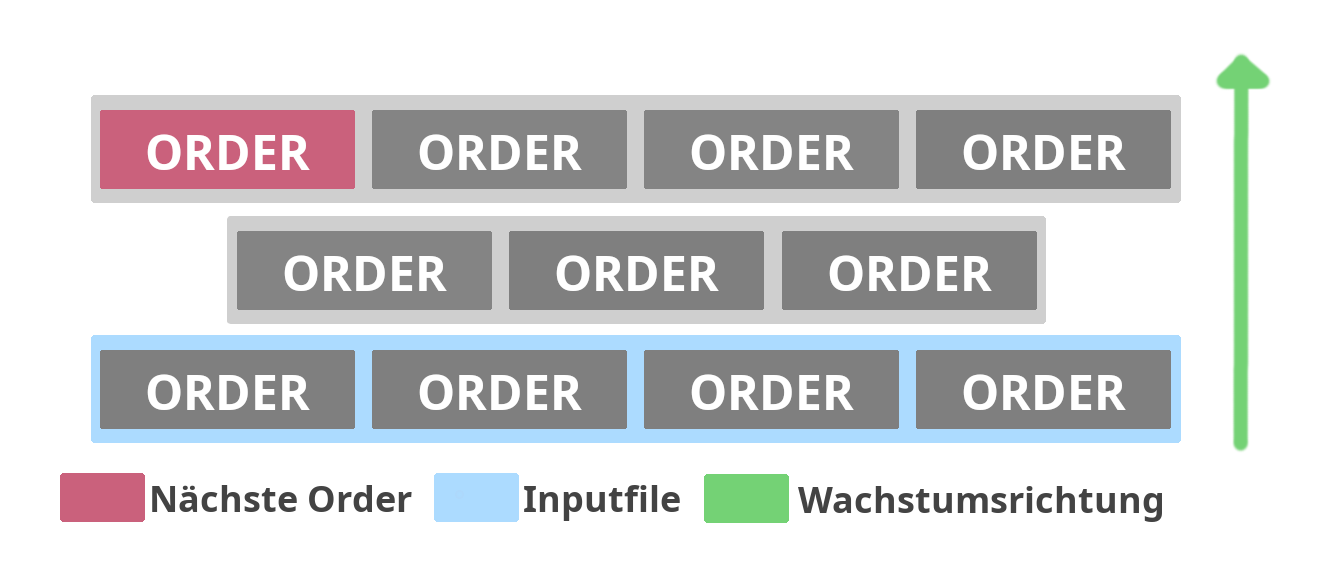
\includegraphics[scale=1.1]{resources/images/fetch-stack.png}
    \caption{Struktur des FetchStacks}
    \label{fig:fetchstack}
\end{figure}

Die Hauptanwendung des FetchStacks wird im Abschnitt \ref{sec:qhs-execute} ausgeführt.
Die Kompilierung wird beendet, sobald keine Order mehr auf dem FetchStack übrig ist.

\section{Validate} \label{sec:qhs-Validate}
Nachdem die nächste Order gefunden wurde, wird diese an Validate weitergegeben. Während dem Validate Schritt kommt die \textit{OrderQueue} ins Spiel. Hierbei handelt es sich, wie der Name schon sagt, um eine Queue an Orders.
Die Aufgabe der OrderQueue ist das Speichern und spätere Zurückholen von Orders. Die OrderQueue kann mithilfe von Instructions, die im Abschnitt \ref{sec:qhs-execute} weiter ausgeführt werden, aktiviert und deaktiviert werden.
Wenn nun eine Order in den Validate Schritt gelangt und die OrderQueue aktiviert ist, wird diese Order der OrderQueue hinzugefügt. Der Execute Schritt wird danach übersprungen und der QHS-Zyklus beginnt von neuem bei Fetch.
Die Order wurde ohne ausgeführt zu werden auf der OrderQueue gespeichert. Später ist es nun möglich diese Order mithilfe von Instructions, die im Abschnitt \ref{sec:qhs-execute} weiter thematisiert werden, 
von der OrderQueue zu entfernen und auszuführen. Bestimmte Instructions und Identifiers können jedoch OrderQueue-Proof, also immun gegen die OrderQueue, gemacht werden. Diese werden, auch wenn die OrderQueue aktiv ist, 
normal an Execute weitergegeben. Dies ist zum Beispiel besonders bei der Instruction, die die OrderQueue wieder deaktiviert, wichtig. Da diese Instruction sonst nicht ausgeführt und somit die OrderQueue nie mehr deaktiviert wird.
LiteralCode kann nicht CodeQueue-Proof sein.

MAYBE CODESTACK FIGURE

Ist die OrderQueue deaktiviert oder die Order OrderQueue-Proof, wird diese an den letzten Schritt Execute weitergegeben.

\section{Execute} \label{sec:qhs-execute}
Execute ist der letzte Schritt des QHS-Zyklus. Hier wird nun auch endlich der tatsächliche Assembly Code generiert. Je nach Typ der Order, Identifier, Instruction oder LiteralCode, läuft Execute sehr unterschiedlich ab.

\subsection{Identifier}
Ein Identifier ist eine Zusammenfassung von mehreren Orders. Diese sind in einem \textit{Environment} definiert.
Hierbei handelt es sich um eine einfach Map, die einen Identifier mit einer Queue an Orders verknüpft.
In anderen Programmiersprachen werden Environments auch als Scope bezeichnet.
Wenn nun ein Identifier in den Execute Schritt kommt, werden die dazugehörige Queue an Orders auf den FetchStack aus Abschnitt \ref{sec:qhs-fetch} gelegt.
Beim nächsten Fetch werden nun die zum Identifier gehörenden Orders zurückgegeben. Um Grunde wird der Identifier mit seinen Orders ersetzt.

Environments sind hierbei in einer Linked-List gespeichert. Somit können neue Environments zu dieser Liste hinzugefügt und von der Liste entfernt werden.
Das unterste Environment der Liste ist hierbei das älteste und das oberste Environment das neuste.
Ein neuer Identifiers wird immer zum obersten Environment hinzugefügt. Definitionen des gleichen Identifiers in älteren Environments werden nicht überschrieben oder gelöscht.
Bei der Abfrage nach einem Identifier wird immer die neuste vorhandene Definition zurückgegeben. Ist keine vorhanden, wird ein Error ausgegeben.

\subsection{LiteralCode}
LiteralCode ist der Weg wie der QHScompiler Assembly Code generiert. Dieser ist sehr simpel. Wenn LiteralCode in den Execute Schritt gelangt, wird alles was zwischen den " Zeichen steht in das Output-Dokument geschrieben.
Dies ist die einzige Möglichkeit für den QHScompiler Assembly Code zu generieren. Somit könnte nur durch das Ändern von den einzelnen LiteralCode Orders die Output-Sprache des QHScompilers komplett geändert werden.

\subsection{Instructions}
Instructions sind die komplexesten Orders für den Execute Schritt. Für jede Instruction ist im QHScompiler eine Funktion definiert, die ausgeführt wird, wenn diese Instruction in den Execute Schritt gelangt.
Diese Funktionen können Variablen im QHScompiler speichern, die OrderQueue aktivieren, Identifier definieren und natürlich noch viel mehr. Folgend sind ein paar der wichtigsten Instructions aufgelistet:

\begin{table}[H]
    \centering
    \caption{Wichtige Instructions des QHScompilers}
    \vspace{3mm} % Adjust the height of the space between caption and tabular
    
    \begin{tabularx}{\textwidth}{l|X}
    \textbf{\#enterOrderQueue}      & Aktiviert die OrderQueue. \\ \hline
    \textbf{\#exitOrderQueue}       & Deaktiviert die OrderQueue. \\ \hline
    \textbf{\#assign}               & Die erste Order der OrderQueue muss ein Identifier sein. Der Rest der Orders auf der OrderQueue wird als Definition für diesen Identifier festgelegt. \\ \hline
    \textbf{\#assignToOne}          & Wie \#assign, jedoch wird nach dem Identifier nur eine weitere Order von der OrderQueue genommen und als Definition für den Identifier verwendet. \\ \hline
    \textbf{\#force}                & Die nächste Order wird nach Fetch sofort an Execute weitergegeben. Überspringt Validate und somit die OrderQueue. \\ \hline
    \textbf{\#lightForce}           & Ähnlich wird \#force, jedoch wird diese nur ausgeführt, wenn \textbf{explain this cuz they don't know OrderQueue depth} \\ \hline
    \textbf{\#orderEnqueue}         & Die nächste Order wird sofort der OrderQueue hinzugefügt, auch wenn diese Order OrderQueue-Proof wäre. Execute wird übersprungen. \\ \hline
    \textbf{\#orderFrontEnqueue}    & Ähnlich wie \#orderEnqueue. Die Order wird jedoch auf den obersten Platz der OrderQueue gesetzt. \\ \hline
    \textbf{\#deepFetch}            & Die erste Order der zweitobersten Liste auf dem FetchStack wird oben auf den FetchStack gesetzt. Ermöglicht den Zugriff auf den Inputfile innerhalb eines Identifiers. \\ \hline
    \textbf{\#queueFetch}           & Die oberste Order der OrderQueue wird oben auf den FetchStack gesetzt \\ \hline 
    \textbf{\#pushEnv}              & Ein neues Environment wird der Environment Linked-List hinzugefügt. \\ \hline
    \textbf{\#popEnv}               & Das neuste Environment der Environment Linked-List wird gelöscht. \\ \hline
    \textbf{\#addLiterals}          & Die beiden obersten Orders auf der OrderQueue müssen LiteralCode sein. Diese werden als Zahl interpretiert und addiert. Sollten diese keine Zahl sein, wird ein Fehler gemeldet.        
    \end{tabularx}
\end{table}

Der QHScompiler umfässt \textbf{33} Instructions, wobei \textbf{5} dieser nur für Debugging des Compilers dienen.

\section{Bringing it all together} \label{sec:qhs-bringing-it-together}
Und das war's. Dies ist der gesamte QHScompiler. Im Vergleich zu einem traditionellen Compiler wirkt der QHScompiler fast schon zu simpel. Und dies hat einen einfachen Grund. Der QHScompiler ist zwar komplett,
die dazugehörige Sprache QHS jedoch noch lange nicht. Es ist zwar grundsätzlich durch LiteralCode möglich jedes Programm zu schreiben und zu kompilieren, jedoch handelt es sich dann dabei einfach nur um Assembly Code.
Doch der Aufbau des QHScompilers ermöglicht es mithilfe von Identifiern eine komplexere Programmiersprache zu definieren.

\subsection{Abkürzungen}
Um die Leserlichkeit von QHS zu verbessern, werden ein paar Identifiers anstelle der umständlichen Instruction Namen definiert.

{
\begin{table}[H]
    \centering
    \caption{Abkürzende Identifier}
    \vspace{3mm} % Adjust the height of the space between caption and tabular
    
    % select font of listing in first column (to be equivalent to listings)
    \begin{tabular}{>{\listingFont\selectfont}l|l}
    \textbf{{[}}                 & \#enterOrderQueue              \\ \hline
    \textbf{{]}}                 & \#exitOrderQueue               \\ \hline
    \textgreater{}\textgreater{} & \#assign                       \\ \hline
    \textbf{-\textgreater{}}     & \#assignToOne                  \\ \hline
    \textbf{!}                   & \#force                        \\ \hline
    \textbf{?!}                  & \#lightForce                   \\ \hline
    \textbf{\textbackslash{}n}   & Eine neue Zeile im Outputdatei
    \end{tabular}
\end{table}
}

Weiter wird in den Kommentaren innerhalb der Beispiele Pseudo-Code verwendet, um den QHS Code besser zu erklären. Kommentare können über mehrere Zeilen reichen und beginnen immer mit /* und enden mit */.
Der Kommentar /* X = "hello" \#pushEnv */ würde bedeuten, dass der Identifier X zu den Orders "hello" (LiteralCode) und \#pushEnv (Instruction) definiert wurde. 

Auch wird besonders bei längeren Identifier Definitionen zuerst der Identifier Name getrennt von den restlichen Orders der OrderQueue hinzugefügt. Diese Seperation dient lediglich der Leserlichkeit und ist ansonsten nicht nötig.

\subsection{Identifier Parameter und Rückgabewert}
Mithilfe der \#enterOrderQueue und \#exitOrderQueue Instructions kann innerhalb eines Identifiers die OrderQueue verwendet werden. Dies ermöglicht eine Art von Parametern und Rückgabewert für Identifier.
Parameter werden vor dem Aufruf eines Identifiers der OrderQueue hinzugefügt. Diese kann dann der Identifier verwenden. Genauso kann der Identifier am Ende Orders der OrderQueue hinzufügen und diese somit zurückgeben.

\begin{lstlisting}[language=QHS, caption=Parameter und Rückgabewert eines Identifiers]
[ foo ]
[
    #orderFrontEnqueue param1 ->    /* param1 = erstes Argument */
    #orderFrontEnqueue param2 ->    /* param2 = zweites Argument */

    param1 " : " param2 \n          /* param1 + " : " + param2 + "\n" */

    [ "return" ]                    /* "return" wird der OrderQueue hinzugefügt */
] >>

[ "1" "2" ]                         /* 2 Argumente werden der OrderQueue hinzugefügt */
foo                                 /* foo wird ausgeführt */
#queueFetch                         /* Die zurückgegebene Order wird von der OrderQueue
                                    geholt und ausgeführt */


%\noindent\hrulefill Output\noindent\hrulefill%
1 : 2
return
\end{lstlisting}


\subsection{Variablen} \label{sec:qhs-vars}
Die Umsetzung von Variablen in QHS ist simpel. Zuerst soll der Assembly Code für das Abziehen der Grösse der Variable vom Stack-Pointer hinzugefügt werden.
Dann wird für die Variable ein Identifier definiert, der zu der Position der Variable auf dem Stack zeigt.
Mit nur LiteralCode in QHS lässt sich dies wie folgt ausdrücken:

\begin{lstlisting}[language=QHS, caption=Definition einer Variable mit viel LiteralCode]
"sub rsp, 4" \n
[ a "[rbp-4]" ] >>      /* a = "[rbp-4]" */

"add " a ", 5"

%\noindent\hrulefill Output\noindent\hrulefill%
sub rsp, 4
add [rbp-4], 5
\end{lstlisting}

Jedoch ist dies noch nicht besonders angenehm. Weiter lässt sich zum Beispiel ein \textit{var} Identifier definieren, der die Grösse der Variable als Argument über die OrderQueue annimmt. Um die in vielen Programmiersprachen geläufige Syntax
einer Variable beizubehalten, wird der Name der Variable mithilfe der \#deepFetch Instruction beschafft.

\begin{lstlisting}[language=QHS, caption=Definition einer Variable mit \textit{var} Identifier]
[ var ]
[
    #orderFrontEnqueue size ->          /* size = argument1 */
    [ name ?! #deepFetch ] >>           /* name = Was nach dem var Identifier folgt */

    "sub rsp, " size \n

    [ ?! name "[rbp-4]" ] >>            /* var = "[rbp-4]" */
] >> 

[ "4" ] var a 

"add " a ", 5"
    
%\noindent\hrulefill Output\noindent\hrulefill%
sub 4
add [rbp-4], 5
\end{lstlisting}

Ganz so richtig funktioniert dies aber noch nicht. Momentan erhält jede Variable die Addresse rbp-4 und somit überschreiben sich die Variablen gegenseitig. Der momentane rbp-Offset muss also gespeichert und erhöht werden.
Hierzu wird bereits am Anfang des Programms ein Identifier rbpOffset als 0 definiert. Mithilfe der \#addToIdentifier Instruction, lässt sich daraufhin rbpOffset erhöhen. Dies kann folgendermassen aussehen:

\begin{minipage}{\linewidth}
\begin{lstlisting}[language=QHS, caption=Definition einer Variable mit rbpOffset]
[ rbpOffset "0" ] >>                    /* rbpOffset = "0" */

[ var ]
[
    #orderFrontEnqueue size ->          /* size = argument1 */
    [ name ?! #deepFetch ] >>           /* name = Was nach dem var Identifier folgt */

    "sub rsp, " size \n

    [ rbpOffset ?! size ] #addToIdentifier      /* rbpOffset += size */

    [ ?! name "[rbp-" ?! rbpOffset "]" ] >>     /* var = "[rbp-OFFSET]" */
] >> 

[ "4" ] var a 
[ "8" ] var b 

"add " a ", 5"
"sub " b ", 10"
    
%\noindent\hrulefill Output\noindent\hrulefill%
sub rsp, 4
sub rsp, 8
add [rbp-4], 5
sub [rbp-12], 10
\end{lstlisting}
\end{minipage}

Zuletzt lässt sich das umständliche Hinzufügen der Grösse der Variable sowie der \textit{var} Identifier unter einem Identifier zusammenfassen. Dies wäre passenderweise die bekannte Bezeichnung für den Typen der Variable.

\begin{lstlisting}[language=QHS, caption=Definition einer Variable mit \textit{int} Identifier]
(...)

[ int ] 
[
    [ "4" ] var
] >>
    
int a 
int b 
    
"add " a ", 5"
"sub " b ", 10"
        
%\noindent\hrulefill Output\noindent\hrulefill%
sub rsp, 4
sub rsp, 8
add [rbp-4], 5
sub [rbp-12], 10
\end{lstlisting}

So sieht eine Variable genau so aus, wie es in anderen Programmiersprachen gebräuchlich ist.

\subsection{Funktionen} \label{sec:qhs-funcs}
Funktionen sind im Vergleich zu Variablen deutlich komplizierter. Hierbei sollen zwei der Problematiken an Funktionen behandelt werden.

Zum Schluss sollte eine Funktionsdefinition wie folgt aussehen:


\begin{lstlisting}[language=C, label=eg:qhs-function_goal, caption=Ziel für die Definition einer Funktion in QHS]
int foo ( int param1 , int param2 )
{
    (...)
}
\end{lstlisting}

Hier lässt sich bereits ein erstes Problem feststellen. Im vorherigen Abschnitt \ref{sec:qhs-vars} wurde der \textit{int} Identifier für die Definition einer Variable verwendet. 
Das int aus Beispiel \ref{eg:qhs-function_goal} würde vom QHScompiler also als Definition für eine Variable verstanden werden. Der Unterschied zwischen Variable und Funktionsdefinition besteht hierbei in den Klammern,
die auf den Namen folgen. Der QHScompiler müsste also beim \textit{int} Identifier nach vorne schauen, ob sich eine Klammer nach dem Namen befindet, und folglich eine Variable oder Funktionsdefinition ausführen.
Dies ist jedoch aufgrund des einfachen Designs des QHScompilers nicht möglich. Er kann bloss Orders ausführen, nicht jedoch überprüfen, ob eine Order vorhanden ist. Glücklicherweise lässt sich dieses Problem jedoch lösen,
ohne eine Änderung am QHScompiler vorzunehmen. Die Lösung basiert darauf beim \textit{int} Identifier sowohl eine Variable als auch eine Funktionsdefinition vorzubereiten, aber keine der beiden bereits auszuführen.
Weiter wird nun eine Klammer als Identifier für eine Funktionsdefinition gesetzt, sowie ein Semikolon für die Definition einer Variable. Befindet sich nach dem Namen also eine Klammer, wird eine Funktionsdefinition ausgeführt.
Ist dort aber ein Semikolon wird eine Variable definiert. Dieses Konzept wird im weiteren als \textit{DelayedExecute} bezeichnet. Das ganze könnte dann wie folgt aussehen:

%minipage keeps the listing from splitting onto multiple pages
\begin{minipage}{\linewidth}
\begin{lstlisting}[language=QHS, caption=Implementation eines DelayedExecute für Definitionen]
[ function ]
[
    #orderFrontEnqueue returnSize ->        /* size = argument1 */
    #orderFrontEnqueue name ->              /* name = argument2 */

    [ ?! name ] #orderToLiteral ":" \n      /* "foo:" */
] >>

[ definition ]
[
    #orderFrontEnqueue size ->          /* size = argument1 */
    [ name ?! #deepFetch ] >>           /* name = Was nach dem var Identifier folgt */

    [ ; ]
    [
        [ #orderEnqueue ! size #orderEnqueue ! name ] var 
    ] >>
    /* ; = [ size name ] var */

    [ ( ]
    [
        [ #orderEnqueue ! size #orderEnqueue ! name ] function 
    ] >>
    /* ( = [ size name ] function */

] >>

[ int ]
[
    [ "4" ] definition
] >>
\end{lstlisting}
\end{minipage}


Das zweite Problem sind die Parameter eine Funktionsdefinition. Diese sehen genau gleich aus wie eine die Definition einer Variable, sollen jedoch vom QHScompiler anders ausgeführt werden.
Erstens sollte bei einer Parameterdefinition nicht der LiteralCode zur Subtraktion vom RSP hinzugefügt werden. Zweitens verwendet eine Parameterdefinition einen anderen rbp-Offset.
Die Lösung hierzu liegt im Umdefinieren des \textit{definition} Identifiers. Dieser ist momentan für sowohl für Variable als auch Funktionsdefinitionen verantwortlich.
Bei der Anfangsklammer der Funktionsdefinition wird der \textit{definition} Identifier neu definiert, sodass er eine Parameterdefinition ausführt. Die vorherige Definition geht dank der \#pushEnv Instruction nicht verloren.
Bei der schliessenden Klammer wird \#popEnv durchgeführt, und der \textit{definition} Identifier ist wieder für Variablen und Funktionen zuständig. Diese Lösung wird im folgenden \textit{TempAssign} genannt.
Dies lässt sich in QHS wie folgt umsetzten:

\begin{minipage}{\linewidth}
\begin{lstlisting}[language=QHS, caption=Implementation eines TempAssigns für Parameter Definitionen]
[ function ]
[
    #pushEnv

    #orderFrontEnqueue returnSize ->        /* size = argument1 */
    #orderFrontEnqueue name ->              /* name = argument2 */

    [ ?! name ] #orderToLiteral ":" \n      /* "foo:" */

    [ definition paramDefinition ]          /* definition = paramDefinition */

    #popEnv             /* Umdefinition von definition wird vergessen */
] >>
\end{lstlisting}
\end{minipage}

Der Identifier \textit{paramDefinition} ist hierbei gleich wie der \textit{var} Identifier aus Abschnitt \ref{sec:qhs-vars}. Jedoch wird anstelle von \textit{rbpOffset} ein neuer \textit{paramOffset} Identifier verwendet.

Nun fehlt nur noch eine Sache für die Funktionsdefinition, der Funktionsbody. Dieser ist vergleichsweise simpel. Die beiden geschwungenen Klammern werden ganz einfach zu einem leeren Identifier definiert und somit einfach ignoriert.
Der gesamte Code innerhalb des Body wird nun einfach ganz normal vom QHScompiler ausgeführt und an den Outputdatei angehängt. Das Endresultat sieht wie folgt aus:

\begin{lstlisting}[language=QHS, caption=Finale Definition einer Funktion in QHS]
int foo ( int param1 , int param2 )
{
    "add " param1 ", " param2
}

%\noindent\hrulefill Output\noindent\hrulefill%
foo:
add [rbp+16], [rbp+20]
\end{lstlisting}

Mithilfe von DelayedExecute und TempAssign lassen sich also auch syntaktisch komplexen Code problemlos in QHS definieren und ausführen.
\textbf{Wie das Callen von Funktionen aussieht, soll hierbei nicht weiter betrachtet werden.}


    






